\pdfminorversion=6
\pdfcompresslevel=9
\pdfobjcompresslevel=2

\documentclass[german,pdftex,dvipsnames,leqno]{beamer}% handout option disables overlays
\mode<presentation>{\usetheme{JK}}

\usepackage[utf8]{inputenc}
\usepackage{babel}
\usepackage[T1]{fontenc}
\usepackage{lmodern} % HACK! This is a workaround for a bug in beamer that triggers in texlive 2017 with \tiny font, which in beamer goes to the untested/unsupported <5pt font (font generation of ecss0400 fails)

\usepackage{amsmath}

% Times/Helvetica/Courier combination
%\usepackage{mathptmx}
%\usepackage[scaled=.90]{helvet}
%\usepackage{courier}

% Palatino/Helvetica/Courier combination
%\usepackage{mathpazo}
%\usepackage[scaled=.95]{helvet}
%\usepackage{courier}

% Formatting
\usepackage{tabto} % provides \tab command
%\usepackage{multicol}

% Disable footnote ruler
\renewcommand{\footnoterule}{}

% Drawing
\usepackage{tikz}
% \usetikzlibrary{positioning,calc,decorations.pathreplacing}
% \usepackage{calc}
% \def\checkmark{\tikz\fill[scale=0.4](0,.35) -- (.25,0) -- (1,.7) -- (.25,.15) -- cycle;}
% \def\scalecheck{\resizebox{\widthof{\checkmark}*\ratio{\widthof{x}}{\widthof{\normalsize x}}}{!}{\checkmark}}

% \tikzstyle{every picture}+=[remember picture]
% \tikzstyle{na} = [baseline=-.5ex]

% \newcommand{\tikzmark}[1]{\tikz[overlay,remember picture] \node (#1) {};}

\usepackage{xcolor}

\newcommand<>\mhl[2][gray!20]{\alt#3{\colorbox{#1}{$#2$}}{\colorbox{white}{$#2$}}} % highlights with box (default light gray) on specified overlay, the white box ensures stable spacing on other slides
\newcommand{\mphbox}[1]{\colorbox{white}{$#1$}} % creates a plain white box to obtain uniform spacing when \mhl is used


%colors from theme
\definecolor{sbdcyan}{RGB}{026, 058, 107}
\definecolor{sbmcyan}{RGB}{038, 116, 176}
\definecolor{sblcyan}{RGB}{109, 182, 218}
\definecolor{greenblue}{RGB}{0, 127, 79}
\definecolor{darkred}{RGB}{128, 0, 0}
\definecolor{darkyellow}{RGB}{128, 128, 0}

% Packages specific to the content
\usepackage{mathpartir}
\usepackage{xspace}
% \usepackage{ntheorem}

% for Inkscape overlays
\usepackage[absolute,overlay]{textpos}
\setlength{\TPHorizModule}{\paperwidth}
\setlength{\TPVertModule}{\paperheight}
\textblockorigin{0mm}{0mm}

%%% MY MACROS, copy old if needed

% Formatting
\newcommand{\hl}[1]{\emph{\color{sbmcyan} #1}}
\newcommand{\mycite}[1]{{\color{gray}\scriptsize[#1]}}

% basic math
\newcommand{\NN}{\ensuremath{\mathbb{N}}}

% spacing
\newcommand{\ms}{\;\,}
\newcommand{\mbin}[1]{\mathbin{\ms #1 \ms}}
\newcommand{\mrel}[1]{\mathrel{\ms #1 \ms}} % meta level binary relation

% meta operators
\newcommand{\mForall}[1]{\forall #1.\ms}
\newcommand{\mExists}[1]{\exists #1.\ms}
\newcommand{\mIff}{\mrel{\iff}}
\newcommand{\mImpl}{\mrel{\Rightarrow}}
\newcommand{\mOf}{\mrel{:}}
\newcommand{\mAnd}{\mrel{\wedge}}
\newcommand{\mOr}{\mrel{\vee}}

% definitions
\newcommand{\eqdef}{\mbin{:=}}
\newcommand{\bnfdef}{\mbin{::=}}

% substitutions
\newcommand{\subst}[1]{\hphantom{|}\![{#1}]}
\newcommand{\id}{\mathsf{id}}
\newcommand{\shift}{\ensuremath{\uparrow}}
\newcommand{\up}{{\Uparrow}}
\newcommand{\scons}{\mathbin{\cdot}}
\newcommand{\scomp}{\mathbin{\circ}}

% adjusting relations
\newcommand{\cons}{\mathbin{\,:\hspace{-0.1em}:\,}}
\newcommand{\rup}[1]{\ensuremath{{#1}^\Uparrow}}
\newcommand{\rext}[1]{\ensuremath{{#1}^{\mathsf{ext}}}}

% systems
\newcommand{\SysF}{\ensuremath{\mathsf{\color{greenblue}F}}\xspace}
\newcommand{\SysL}{\ensuremath{{\color{sbmcyan}\lambda2}}\xspace}

\newcommand{\ty}{\mathsf{ty}}
\newcommand{\tm}{\mathsf{tm}}

% syntax
\newcommand{\TyF}{\ensuremath{\mathsf{\color{greenblue}Ty_{F}}}}
\newcommand{\TmF}{\ensuremath{\mathsf{\color{greenblue}Tm_{F}}}}

\newcommand{\impf}[2]{\ensuremath{#1 \mathbin{\color{greenblue}\rightarrow} #2}}
\newcommand{\allf}[1]{\ensuremath{{\color{greenblue}\forall.} #1}}
\newcommand{\nallf}[2]{\ensuremath{{\color{greenblue}\forall} #1 {\color{greenblue}.} #2}}
%\newcommand{\appf}[2]{\ensuremath{#1 \mathop{\color{greenblue}\$} #2}}
\newcommand{\appf}[2]{\ensuremath{#1 \; #2}}
\newcommand{\lamf}[2]{\ensuremath{{\color{greenblue}\lambda} #1 {\color{greenblue}.} #2}}
%\newcommand{\tyappf}[2]{\ensuremath{#1 \mathop{\color{greenblue}@} #2}}
\newcommand{\tyappf}[2]{\ensuremath{#1 \; #2}}
\newcommand{\tylamf}[1]{\ensuremath{{\color{greenblue}\Lambda.}#1}}
\newcommand{\ntylamf}[2]{\ensuremath{{\color{greenblue}\Lambda} #1 {\color{greenblue}.} #2}}

\newcommand{\TmL}{\ensuremath{\mathsf{\color{sbmcyan}Tm_{\lambda}}}}

\newcommand{\typl}{\ensuremath{{\color{sbmcyan}\square}}}
\newcommand{\prpl}{\ensuremath{\textrm{\color{sbmcyan}\textasteriskcentered}}}
%\newcommand{\appl}[2]{\ensuremath{#1 \mathop{\color{sbmcyan}\$} #2}}
\newcommand{\appl}[2]{\ensuremath{#1 \; #2}}
\newcommand{\laml}[2]{\ensuremath{{\color{sbmcyan}\lambda} #1 {\color{sbmcyan}.} #2}}
\newcommand{\prodl}[2]{\ensuremath{{\color{sbmcyan}\Pi} #1 {\color{sbmcyan}.} #2}}

% judgements
\newcommand{\of}{\mathbin{:}}
\newcommand{\tsf}{\mathrel{\color{greenblue}\vdash}}
\newcommand{\tsl}{\mathrel{\color{sbmcyan}\vdash}}

\newcommand{\istyf}[1]{\ensuremath{#1 \ms \mathbf{\color{greenblue}ty}}}
\newcommand{\typingf}[2]{\ensuremath{#1 \mathrel{\color{greenblue}\of_{\mathsf{F}}} #2}}

\newcommand{\univl}[1]{\ensuremath{\mathcal{\color{sbmcyan}U}\, #1}}
\newcommand{\typingl}[2]{\ensuremath{#1 \mathrel{\color{sbmcyan}\of_{2}} #2}}

\newcommand{\tyrel}[2]{\ensuremath{#1 \mathrel{\sim} #2}}
\newcommand{\tmrel}[2]{\ensuremath{#1 \mathrel{\approx} #2}}

% relational context morphisms
\newcommand{\tyctxrelFL}[3]{\ensuremath{#1\mathrel{\mathop{\longrightarrow}^{#2}\limits}#3}}
\newcommand{\tyctxrelLF}[3]{\ensuremath{#1\mathrel{\mathop{\longleftarrow}^{#2}\limits}#3}}
\newcommand{\tmctxrelFL}[4]{\ensuremath{#1\mathrel{\mathop{\longrightarrow}^{#2}_{#3}\limits}#4}}
\newcommand{\tmctxrelLF}[4]{\ensuremath{#1\mathrel{\mathop{\longleftarrow}^{#2}_{#3}\limits}#4}}

% LambdaProlog symbols
\newcommand{\lpProp}{\ensuremath{\mathbf{o}}}
\newcommand{\lpPi}[1]{\boldsymbol{\Pi} #1.\ms}
\newcommand{\lpApp}[2]{#1\langle#2\rangle}
\newcommand{\lpImp}{\mrel{=\!\blacktriangleright}}

% G Symbols
\newcommand{\gProp}{\ensuremath{\mathbf{Prop}}}

\DeclareMathOperator\ham{ham}

%%% END MACROS

% Generate Section Title Pages
% \AtBeginSection{\frame[noframenumbering]{\sectionpage}}
% \setbeamertemplate{section page}
% {
%   \begin{centering}
%     \begin{beamercolorbox}[sep=4pt,center]{part title}
%       \usebeamerfont{section title}\insertsection\par
%     \end{beamercolorbox}
%   \end{centering}
% }

%%%%%%%%%%%%%%%%%%%%%%%%%%%%%%%%%%%%%%%%%%%%%%%%%%%%%%%%%%%%%%%%%%%%%%%%%%%%%%%%
% Metadata
%%%%%%%%%%%%%%%%%%%%%%%%%%%%%%%%%%%%%%%%%%%%%%%%%%%%%%%%%%%%%%%%%%%%%%%%%%%%%%%%
\title[Aktorenmodell und Skalierbarkeit]{Aktorenmodell und Skalierbarkeit}
%\subtitle{}

\author[Jonas Kaiser]{
  \texorpdfstring{
    Jonas Kaiser
  }
  {Jonas Kaiser}}

%\institute[Saarland University]{\normalsize FSCD 2017, Oxford}

\date{19. Oktober 2018}

%%%%%%%%%%%%%%%%%%%%%%%%%%%%%%%%%%%%%%%%%%%%%%%%%%%%%%%%%%%%%%%%%%%%%%%%%%%%%%%%
% Content
%%%%%%%%%%%%%%%%%%%%%%%%%%%%%%%%%%%%%%%%%%%%%%%%%%%%%%%%%%%%%%%%%%%%%%%%%%%%%%%%

\begin{document}

\section*{Introduction}

\begin{frame}[plain]
  \titlepage
\end{frame}

\begin{frame}
  \frametitle{Wer bin ich, \ldots}
  \begin{columns}
    \column{0.48\linewidth}
    \structure{Gebürtiger Münsteraner}
    \begin{center}
      
\includegraphics[scale=0.15]{img/bicycle}
    \end{center}
    \structure{Informatik Studium / Promotion}
    \begin{itemize}
    \item 2010 -- BA, Cambridge, UK
    \item 2013 -- MSc, Saarbrücken
    \item \textit{bald} -- PhD, Saarbrücken
    \end{itemize}
    \structure{Wechsel in die Wirtschaft}
    \begin{itemize}
    \item Seit Juni -- dataWerks GmbH
    \end{itemize}
    \column{0.48\linewidth}
    \centering
    \includegraphics[scale=0.30]{img/europe-jk}
  \end{columns}
\end{frame}

\begin{frame}
  \frametitle{\ldots und wofür schlägt mein Herz?}
  \begin{center}
    \includegraphics<1>[scale=0.4]{img/mmV1}
    \includegraphics<2>[scale=0.4]{img/mmV2}
    \includegraphics<3>[scale=0.4]{img/mmV3}
    \includegraphics<4>[scale=0.4]{img/mmV4}
    \includegraphics<5>[scale=0.4]{img/mmV5}
    \includegraphics<6>[scale=0.4]{img/mmV6}
  \end{center}
\end{frame}

% \begin{frame}
%   \frametitle{Overview}
%   \tableofcontents
% \end{frame}

% \section{Variants of System F}

% \begin{frame}
%   \frametitle{System F \mycite{Girard '72} / PTLC \mycite{Reynolds '74}}
%   \pause
%   \structure{Some History}
%   \begin{itemize}
%   \item Developed in the context of proof theory and polymorphism.
%   \item Commonly phrased as a {\color{greenblue}two-sorted} system: \emph{Types} \& \emph{Terms}
%   \item We consider \SysF as presented in \mycite{Harper '13}.
%     \begin{itemize}
%     \item Explicitly scopes type variables.
%     \end{itemize}
%   \end{itemize}
%   \vspace{1em}
%   \pause
%   \structure{Meanwhile \ldots}
%   \begin{itemize}
%   \item Study of CC led to {\color{sbmcyan}single-sorted} Pure Type Systems (PTS):
%     \begin{itemize}
%     \item The $\lambda$-cube of \mycite{Barendregt '91}.
%     \end{itemize}
%   \item System~F appears as the corner $\SysL$.
%   \end{itemize}
%   \vspace{1em}
%   \pause
%   \begin{block}{Goal: Transport of Results}
%     \vspace{-1em}
%     \begin{center}
%       \pause$\SysF \quad \leftrightsquigarrow \quad\SysL$\\
%       \pause\emph{bidirectional reduction of typing}
%     \end{center}
%     \vspace{-1em}
%   \end{block}
% \end{frame}

% \begin{frame}
%   \frametitle{Related Work}
%   \begin{itemize}
%   \item<2-> The reduction result is partially discussed in \mycite{Geuvers '93}.
%     \begin{itemize}
%     \item Primarily argues the forward preservation of typing.
%     \item The syntactic correspondence is left implicit.
%     \end{itemize}
%   \item<3-> Coq formalisation of the full reduction in \mycite{K/Tebbi/Smolka '17}.
%     \begin{itemize}
%     \item Pairs of translation functions establish the syntactic correspondence.
%     \item Requires involved cancellation laws.
%     \item Proofs based on an extension of context morphism lemmas \mycite{Goguen/McKinna '97, Adams '06}.
%     \end{itemize}
%   \item<4-> Goal of this work:
%     \begin{center}
%       Correspondence Proof as \hl{benchmark}\\ for reasoning about\\ \hl{syntax} and \hl{contextual information}.
%     \end{center}
%   \end{itemize}
% \end{frame}

% \begin{frame}
%   \frametitle{Syntactic Variants $\SysF$ and $\SysL$}
%   \onslide<2->{{\color{greenblue}Two-sorted non-uniform syntax:}}
%   \begin{align*}
%     \onslide<2->{&\TyF & A, B \bnfdef &\mphbox{X} \mid \mhl<4>{\impf{A}{B}} \mid \mhl<4>{\nallf{X}{A}} \\
%     &\TmF & s, t \bnfdef &\mphbox{x} \mid \mhl<6>{\appf{s}{t}} \mid \mhl<5>{\lamf{x \of A}{s}} \mid \mhl<6>{\tyappf{s}{A}} \mid \mhl<5>{\ntylamf{X}{s}}\\[.6em]
%     &\textup{\color{greenblue}Type Formation} & &\Delta \tsf \istyf{A} \\
%     &\textup{\color{greenblue}Typing} & &\Delta; \Gamma \tsf \typingf{s}{A} \\}
%     \onslide<3->{\intertext{\color{sbmcyan}Single-sorted uniform PTS syntax:}
%     &\TmL & a, b \bnfdef &\mphbox{x} \mid \mphbox{\prpl} \mid \mphbox{\typl} \mid \mhl<6>{\appl{a}{b}} \mid \mhl<5>{\laml{x \of a}{b}} \mid \mhl<4>{\prodl{x \of a}{b}}\\[.6em]
%     &\textup{\color{sbmcyan}Typing} & & \Psi \tsl \typingl{a}{b}}
%   \end{align*}
% \end{frame}

% \begin{frame}
%   \frametitle{Syntactic Correspondence}
%   \begin{center}
%     \begin{tikzpicture}
%       %\draw[step=.5cm,gray,very thin] (0,0) grid (12,7);
%       \draw<1->[rounded corners=.5cm,very thick,greenblue] (.5,4.5) rectangle (4.5,6.5);
%       \node<1->[right] at (.75,6.1) {$\TyF$};
%       \draw<2->[dashed,greenblue,thick] (2.5,5.25) ellipse (1.5cm and .5cm);
%       \node<2-> at (2.5,5.25) {\textit{\scriptsize well-formed types}};
%       \draw<1->[rounded corners=.5cm,very thick,greenblue] (.5,1) rectangle (4.5,3.5);
%       \node<1->[right] at (.75,3.1) {$\TmF$};
%       \draw<2->[dashed,greenblue,thick] (2.5,2) ellipse (1.5cm and .75cm);
%       \node<2-> at (2.5,2) {\textit{\scriptsize well-typed terms}};
%       \draw<1->[rounded corners=.5cm,very thick,sbmcyan] (7.5,1) rectangle (11.5,6.5);
%       \node<1->[right] at (7.75,6.1) {$\TmL$};
%       \draw<2->[dashed,sbmcyan,thick] (9.5,5.25) ellipse (1.5cm and .5cm);
%       \node<2-> at (9.5,5.25) {\textit{\scriptsize propositions}};
%       \draw<2->[dashed,sbmcyan,thick] (9.5,2) ellipse (1.5cm and .75cm);
%       \node<2-> at (9.5,2) {\textit{\scriptsize proofs}};
%       \draw<3->[<->,thick,gray] (4,5.25) to[bend left] node[above] {\color{black}$\only<4->{\Theta \vdash}\tyrel{A}{a}$} (8,5.25);
%       \draw<3->[<->,thick,gray] (4,2) to[bend right] node[below] {\color{black}$\only<4->{\Theta; \Sigma \vdash}\tmrel{s}{b}$} (8,2);
%       \draw<5->[sbdcyan,thick] (5,2.15) rectangle (7,5);
%       \node<5->[sbdcyan,right] at (5,4.65) {\scriptsize 1) injective};
%       \node<5->[sbdcyan,right] at (5,4.15) {\scriptsize 2) functional};
%       \node<5->[sbdcyan,right] at (5,3.65) {\scriptsize 3) L-total \&};
%       \node<5->[sbdcyan,right] at (5.35,3.3) {\scriptsize preserving};
%       \node<5->[sbdcyan,right] at (5,2.8) {\scriptsize 4) R-total \&};
%       \node<5->[sbdcyan,right] at (5.35,2.45) {\scriptsize preserving};
%     \end{tikzpicture}
%   \end{center}
% \end{frame}

% \begin{frame}
%   \frametitle{Syntactic Correspondence -- Two Complications}
%   \begin{enumerate}
%   \item<2-> Non-uniform vs.\ uniform:
%     \vspace{.5em}
%     \begin{center}
%       \begin{tikzpicture}
%         %\draw[step=.5cm,gray,very thin] (0,0) grid (11,3);
%         \draw<2->[dotted,very thick,greenblue] (1.5,2.75) -- (1.75,2.75);
%         \draw<2->[rounded corners=.5cm,very thick,greenblue] (1.75,2.75) -- (4.75,2.75) -- (4.75,0.25) -- (1.75,0.25);
%         \draw<2->[dotted,very thick,greenblue] (1.5,0.25) -- (1.75,0.25);
%         \draw<2->[dashed,greenblue,thick] (2.5,1.5) ellipse (2cm and 1cm);
%         \node<4->[left] (L1) at (3.1,2) {$\impf{A}{B}$};
%         \node<5->[left] (L2) at (3.1,1) {$\nallf{X}{B}$};
%         \draw<2->[dotted,very thick,sbmcyan] (9.5,2.75) -- (9.25,2.75);
%         \draw<2->[rounded corners=.5cm,very thick,sbmcyan] (9.25,2.75) -- (6.25,2.75) -- (6.25,0.5);
%         \draw<2->[dotted,very thick,sbmcyan] (6.25,0.5) -- (6.25,0.25);
%         \draw<2->[dashed,sbmcyan,thick] (8.5,1.5) ellipse (2cm and .75cm);
%         \node<3->[right] (R) at (7.75,1.5) {$\prodl{x:a}{b}$};
%         \draw<6->[<->,thick,gray,shorten <= .2cm, shorten >= .2cm] (L1) to[out=10,in=180] (R);
%         \draw<6->[<->,thick,gray,shorten <= .2cm, shorten >= .2cm] (L2) to[out=-10,in=180] (R);
%         \node<6->[red] at (5.5,1.5) {?};
%       \end{tikzpicture}
%     \end{center}
%     \vspace{.5em}
%   \item<7-> Open terms \& contextual assumptions about
%     \begin{itemize}
%     \item<8-> \hl{well-formedness}: \tabto{0.3\linewidth} in $\impf{X}{X}$, is $X$ in scope?
%     \item<9-> \hl{typing}: \tabto{0.3\linewidth} in $\appl{a}{b}$, is $b$ a proof or proposition?
%     \item<10-> \hl{related variables}: \tabto{0.3\linewidth} in the variable case, does  $\Theta \vdash \tyrel{X}{x}$ hold?
%     \end{itemize}
%   % \item<11-> Aligning the binding structures.
%   %   \begin{itemize}
%   %   \item Two variable scopes for \SysF vs.\ unified scope for \SysL.
%   %   \end{itemize}
%   % \item<12-> Example (Polymorphic Identity):
%   %   \begin{align*}
%   %     {} &\vdash \tyrel{\nallf{X}{\impf{X}{X}}}{\prodl{x:\prpl}{\prodl{y:x}{x}}} \\
%   %     {} &\vdash \tmrel{\ntylamf{X}{\lamf{x:X}{x}}}{\laml{y:\prpl}{\laml{z:y}{z}}}
%   %   \end{align*}
%   \end{enumerate}
% \end{frame}

% \begin{frame}
%   \frametitle{The Reduction Proof: $\SysF \leftrightsquigarrow \SysL$}
%   Assume we are given syntactic relations $\sim$ and $\approx$ which are both:
%   \begin{enumerate}
%   \item functional
%   \item injective
%   \item left-total and judgement preserving on suitable fragment
%   \item right-total and judgement preserving on suitable fragment
%   \end{enumerate}
%   \pause
%   \setbeamercovered{transparent}
%   \begin{theorem}[Reduction $\SysF \rightsquigarrow \SysL$]\vspace{-2em}
%     \begin{align*}
%       \onslide<2-4>{{} \tsf \istyf{A} &\mIff \mExists a {} \vdash \tyrel{A}{a} \mAnd {} \tsl \typingl{a}{\prpl}}\\
%       \onslide<2,4>{{} \tsf \typingf{s}{A} &\mIff \mExists{ba} {} \vdash \tmrel{s}{b} \mAnd {} \vdash \tyrel{A}{a} \mAnd {} \tsl \typingl{b}{a} \mAnd {} \tsl \typingl{a}{\prpl}}
%     \end{align*}
%     \vspace{-1.8em}
%   \end{theorem}
%   \begin{theorem}[Reduction $\SysL \rightsquigarrow \SysF$]\vspace{-1.8em}
%     \begin{align*}
%       \onslide<2,4>{{} \tsl \typingl{a}{\prpl} &\mIff \mExists A {} \vdash \tyrel{A}{a} \mAnd {} \tsf \istyf{A}}\\
%       \onslide<2,4>{{} \tsl \typingl{b}{a} \mAnd {} \tsl \typingl{a}{\prpl} &\mIff \mExists {sA} {} \vdash \tmrel{s}{b} \mAnd {} \vdash \tyrel{A}{a} \mAnd {} \tsf \typingf{s}{A}}
%     \end{align*}
%     \vspace{-1.8em}
%   \end{theorem}
% \end{frame}

% \begin{frame}
%   \frametitle{A Separation of Concerns}
%   \structure{The Four Properties}
%   \begin{itemize}
%   \item<2-> Primarily inductive proofs over defined structures.
%   \item<3-> Heavily depends on representation of:
%     \begin{itemize}
%     \item Syntax
%     \item Predicates over Syntax, i.e.\ judgements
%     \end{itemize}
%   \item<4-> May depend on language-local meta-theory (e.g.\ propagation).
%   \item<5-> In general: very specific to the chosen theorem prover.
%   \end{itemize}
%   \vspace{1em}
%   \structure{The Two Reduction Theorems}
%   \begin{itemize}
%   \item<6-> No induction, just basic logic.
%   \item<7-> Relatively straightforward.
%   \item<8-> Essentially agnostic with respect to the theorem prover.
%   \end{itemize}
% \end{frame}



% \begin{frame}
%   \frametitle{Formalising the Proof}
%   \structure<1->{We consider three approaches:}
%   \begin{itemize}
%   \item<2-> Coq \tabto{.2\linewidth} first-order de Bruijn, par. substitutions, invariants
%   \item<3-> Abella \tabto{.2\linewidth} HOAS, $\nabla$-quantification, relational proof search
%   \item<4-> Beluga \tabto{.2\linewidth} HOAS, 1$^{\textit{st}}$-class contexts, context schemas
%   \end{itemize}
%   \vspace{1em}
%   \onslide<5->{\structure{Topics of Interest}}
%   \begin{itemize}
%   \item<6-> Representation of syntax and judgements.
%   \item<7-> Management of local variable binding.
%   \item<8-> Tracking of contextual information.
% %  \item<9-> Adequacy of representation.
%   \item<9-> Technicalities: Usability / Libraries / Tool Support
%   \end{itemize}
% \end{frame}

\section{Aktorenmodell}

\begin{frame}
  \begin{center}
    \begin{Large}
      \hl{-- Aktorenmodell --}
    \end{Large}
  \end{center}
\end{frame}

\begin{frame}
  \frametitle{Ziel: Optimale Auslastung von Resourcen}
  \begin{itemize}
  \item \textbf{Früher:} Multi-Core CPUs, heterogene Prozessor Architektur, Hyperthreading
  \item \textbf{Heute:} Vernetzte Systeme, Cloud
    \begin{itemize}
    \item Physisch: Server, Workstation, Cluster
    \item Virtuell: Dünner Anwendungs-Container bis zum vollvirtualisierten OS
    \end{itemize}
  \end{itemize}
  \pause
  \structure{$\Rightarrow$ Wir brauchen Modelle für Nebenläufigkeit ($=$ logische Parallelität)}
  \vspace{1em}
  \pause
  \begin{block}{Relevante Metriken:}
    \begin{itemize}
    \item Verständlichkeit / Ease of Use
    \item Effizienz
    \item Skalierbarkeit / Elastizität
    \item Fehleranfälligkeit
    \end{itemize}
  \end{block}
\end{frame}

\begin{frame}
  \frametitle{Zwei Modelle: Threads vs.\ Actors}
  \begin{columns}
    \column{0.48\linewidth}
    \begin{center}
      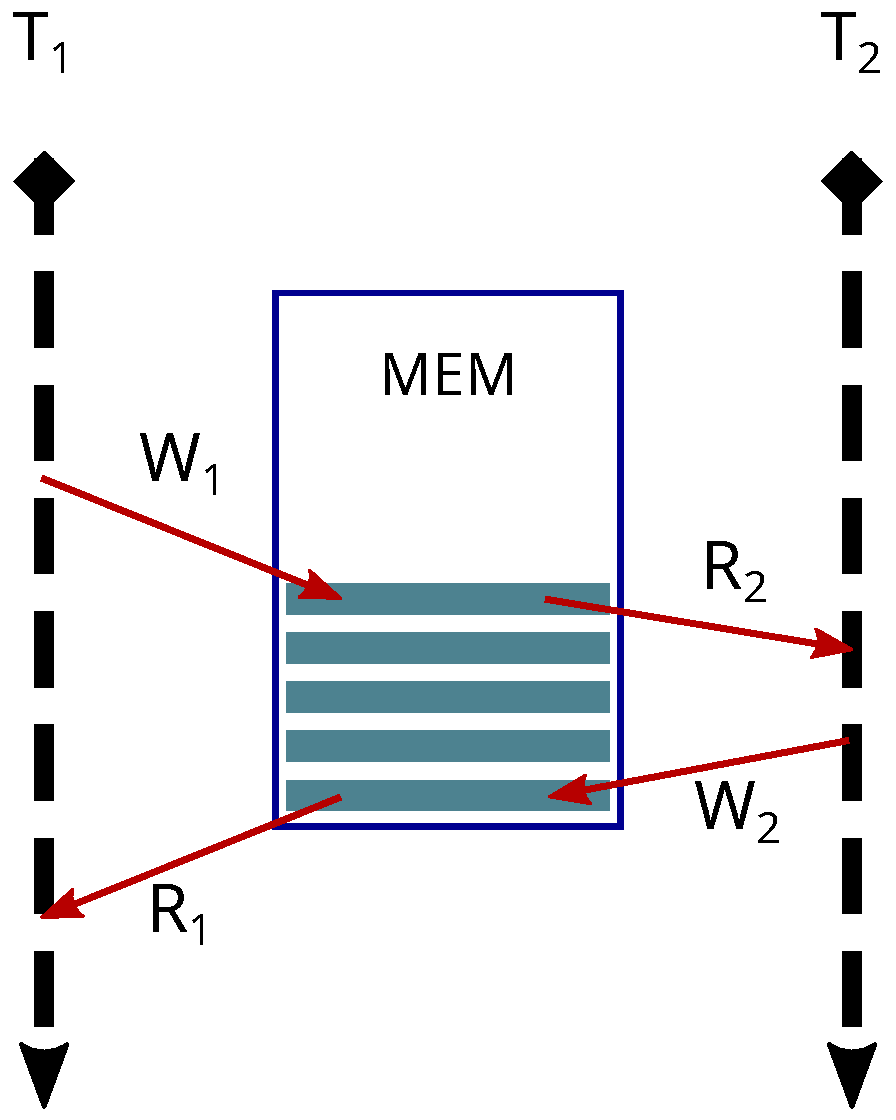
\includegraphics[scale=0.2]{img/threads}
    \end{center}
    \begin{itemize}
    \item Geteilter Speicher
    \item Erfordert Synchronisation
    \item Näher an der Maschine
    \end{itemize}
    \column{0.48\linewidth}
    \begin{center}
      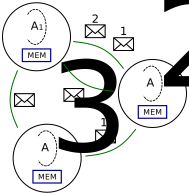
\includegraphics[scale=0.2]{img/actors}
    \end{center}
    \begin{itemize}
    \item Lokaler, privater Speicher
    \item Nachrichtenaustausch (async)
    \item Näher am Menschen
    \end{itemize}
  \end{columns}
\end{frame}

\begin{frame}
  \frametitle{Evaluierung}
  \begin{itemize}
  \item Moderne CPUs haben lokale Caches an jedem Kern
  \item Verteiltes Speichermodell skaliert zu Cloud-Anwendungen
  \item Nachrichtenaustausch ist Grundbaustein (TCP, REST, Mail, \ldots)
  \item Asynchroner Nachrichtenaustausch ist intuitiv
  \item Aktoren sind logisch geschlossene Einheiten
    \begin{itemize}
    \item erleichtert dynamische Topologien
    \item erleichtert Programmierung (weniger Bugs)
    \end{itemize}
  \item Einziger Nachteil: Meist etwas weniger performant aufgrund der zusätzlich erforderlichen Kommunikationsebene.
  \end{itemize}
  \vspace{1em}
  \pause
  \begin{block}{Fazit}
    Das Aktorenmodell ist in fast allen Belangen die bessere Wahl.
  \end{block}
\end{frame}

\section{simLucid}

\begin{frame}
  \begin{center}
    \begin{Large}
      \hl{-- Fallstudie: simLucid --}
    \end{Large}
  \end{center}
\end{frame}


\begin{frame}
  \frametitle{Die Hamming Sequenz als Datenfluss-Diagram}
  Entspricht der gewollten Semantik eines Lucid Programs.
  \begin{center}
    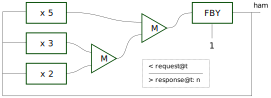
\includegraphics[scale=0.30]{img/hamming}
    \begin{align*}
      \ham &= 1, {\color{sbdcyan}2}, {\color{sbmcyan}3}, {\color{sblcyan}4}, {\color{greenblue}5}, {\color{darkred}6}, {\color{darkyellow}8}, 9, 10, 12, 15, \ldots\\
      \ham x \, 2 &= {\color{sbdcyan}2}, {\color{sblcyan}4}, {\color{darkred}6}, {\color{darkyellow}8}, 10, 12, 16, \ldots\\
      \ham x \, 3 &= {\color{sbmcyan}3}, {\color{darkred}6}, 9, 12, 15, 18, 24, \ldots\\
      \ham x \, 5 &= {\color{greenblue}5}, 10, 15, 20, 25, 30, 40, \ldots\\
    \end{align*}
    \textit{Anm.: Heute würde man hierfür eher eine rekursive Definition in einer funktionalen Sprache wie z.B.\ Haskell wählen.}
  \end{center}
  \begin{itemize}
  \item short intro to dataflow / Lucid (mention that modern functional languages are better suited to these kind of stream programs)
  \item explain dataflow semantics, relate to actor model, highlight scalable design
  \item sketch solution, start from AST, only drop existence of FE/parser as hint
  \item also point out the dynamic unfolding of the network
  \end{itemize}
\end{frame}

% \begin{frame}
%   \frametitle{Coq -- Representation}
%   \begin{itemize}
%   \item<2-> Syntax: first-order de Bruijn
%     \begin{align*}
%       A, B \bnfdef &n_{\color{greenblue}\ty} \mid \impf{A}{B} \mid \allf{A} & &n \in \NN \\
%       s, t \bnfdef &n_{\color{greenblue}\tm} \mid \appf{s}{t} \mid \lamf{A}{s} \mid \tyappf{s}{A} \mid \tylamf{s} & &
%     \end{align*}
%   \item<3-> Typing contexts:
%     \begin{align*}
%       \Delta &\mOf \NN & &\textup{-- \hl{excl.\ upper bound for free type variables}}\\
%       \Gamma &\mOf \mathsf{list}\;\TyF & &\textup{-- \hl{dangling indices reference by position}}
%     \end{align*}
%   \item<4-> Judgements as inductive predicates, e.g.:
%     \begin{align*}
%       \_;\_\tsf\typingf{\_}{\_} \mOf \NN \to \mathsf{list}\;\TyF \to \TmF \to \TyF \to \gProp
%     \end{align*}
%   \item<5-> Parallel substitutions from \hl{Autosubst} library \mycite{Schäfer/Tebbi/Smolka '15}:
%     \begin{align*}
%       \sigma &\of \NN \to \mathcal{T} & (\allf{A})\subst{\sigma} & = \allf{A\subst{\up\sigma}} & \up\sigma &\eqdef 0_{\color{greenblue}\ty} \scons (\sigma\,\scomp \shift)
%     \end{align*}
%   \end{itemize}
% \end{frame}

% \begin{frame}
%   \frametitle{Coq -- Relating Indices}
%   \begin{itemize}
%   \item<2-> Relating open terms requires \hl{explicit} tracking of related indices:
%     \begin{align*}
%       R, S \of \mathsf{list}\;(\NN \times \NN)
%     \end{align*}
%   \item<3-> Traversal of binders requires context adjustments:
%     \begin{mathpar}
%       \inferrule*{R \vdash \tyrel{A}{a} \\ {\color{red}\rup{R}} \vdash \tyrel{B}{b}}{R \vdash \tyrel{\impf{A}{B}}{\prodl{a}{b}}} \and
%       \inferrule*{{\color{red}\rext{R}} \vdash \tyrel{A}{a}}{R \vdash \tyrel{\allf{A}}{\prodl{\prpl}{a}}}
%     \end{mathpar}
%     \vspace{-1em}
%     \onslide<4->{\begin{align*}
%       {\color{red}\rext{R}} &\eqdef (0,0) \cons \mathsf{map}\,\,(\shift \times \shift)\,\,R\\
%       {\color{red}\rup{R}} &\eqdef \mathsf{map}\,\,(\id\, \times \shift)\,\,R\\
%     \end{align*}}
%     \vspace{-1em}
%     \onslide<5->{\begin{mathpar}
%       \inferrule*{R \vdash \tyrel{A}{a} \\ {\color{red}\rup{R};\rext{S}} \vdash \tmrel{s}{b}}{R;S \vdash \tmrel{\lamf{A}{s}}{\laml{a}{b}}}
%     \end{mathpar}}
%   \end{itemize}
% \end{frame}

% \begin{frame}
%   \frametitle{Coq -- Context Management}
%   \onslide<2->{\structure{Functionality of $\sim$}
%   \begin{enumerate}
%   \item $R\;\textit{func} \mImpl \rext{R}\;\textit{func} \mAnd \rup{R}\;\textit{func}$
%   \item $R\;\textit{func} \mImpl (R \vdash \tyrel{\_}{\_})\;\textit{func}$ \tabto{.85\linewidth} \hl{ind.}
%   \end{enumerate}}
%   \vspace{1em}
%   \onslide<3->{\structure{Injectivity of $\approx$}
%   \begin{enumerate}
%   \item $R\;\textit{inj} \mImpl \rext{R}\;\textit{inj} \mAnd \rup{R}\;\textit{inj}$
%   \item Write $R \parallel S$ for $R$ and $S$ having disjoint ranges.
%   \item $R \parallel S \mImpl \rup{R} \parallel \rext{S}$
%   \item $R \parallel S \mImpl \neg (R \vdash \tyrel{A}{a} \mAnd R;S \vdash \tmrel{s}{a})$ \tabto{.85\linewidth} \hl{ind./inv.}
%   \item $R\;\textit{inj} \mImpl S\,\textit{inj} \mImpl R \parallel S \mImpl (R;S \vdash \tmrel{\_}{\_})\;\textit{inj}$ \tabto{.85\linewidth} \hl{ind.}
%   \item Also requires injectivity of $\sim$.
%   \end{enumerate}}
% \end{frame}

% \begin{frame}
%   \frametitle{Coq -- Custom Invariants}
%   \structure{Left-Totality and Preservation of Type Formation of $\sim$}
%   \begin{enumerate}
%   \item<2-> Define Invariant:
%     \begin{align*}
%       \tyctxrelFL{\Delta}{R}{\Psi} \eqdef \mForall{x < \Delta} \mExists y (x,y) \in R \mAnd (\typingl{y}{\prpl}) \mathrel{\in_\lambda} \Psi
%     \end{align*}
%   \item<3-> Prove Extension Laws:
%     \begin{align*}
%       \tyctxrelFL{\Delta}{R}{\Psi} &\mImpl \tyctxrelFL{\Delta}{\rup{R}}{\Psi,a} & &\textup{-- \hl{ext.\ with new term variable}}\\
%       \tyctxrelFL{\Delta}{R}{\Psi} &\mImpl \tyctxrelFL{\Delta+1}{\rext{R}}{\Psi,\prpl} & &\textup{-- \hl{ext.\ with new type variable}}
%     \end{align*}
%   \item<4-> Prove by induction on $\Delta \tsf \istyf{A}$:
%     \begin{align*}
%       \Delta \tsf \istyf{A} \mImpl \mForall {R,\Psi} \tyctxrelFL{\Delta}{R}{\Psi} \mImpl \mExists a R \vdash \tyrel{A}{a} \mAnd \Psi \tsl \typingl{a}{\prpl}
%     \end{align*}
%   \item<5-> Repeat for remaining three preservation results.
%   \end{enumerate}
% \end{frame}

% \begin{frame}
%   \begin{center}
%     \begin{Large}
%       \hl{-- Abella --}
%     \end{Large}\\[2em]
%     HOAS, $\nabla$-quantification, relational proof search
%   \end{center}
% \end{frame}

% \begin{frame}
%   \frametitle{Abella \mycite{Miller, Chaudhuri et al.\ '14}}
%   \structure{Two-level logic:}
%   \begin{itemize}
%   \item<2-> \hl{Specification Level:} $\lambda$Prolog, HOAS, logic predicates, proof search
%     \begin{align*}
%       &\lamf{\_}{\_} \mOf \TyF \to (\TmF \to \TmF) \to \TmF & &\\
%       &\prodl{\_}{\_} \mOf \TmL \to (\TmL \to \TmL) \to \TmL & &\\[.8em]
%       &\typingf{\_}{\_} \mOf \TmF \to \TyF \to \lpProp & &\textup{+ $\lambda$Prolog rules}\\
%       &\tmrel{\_}{\_} \mOf \TmF \to \TmL \to \lpProp & &\textup{+ $\lambda$Prolog rules}
%     \end{align*}
%   \item<3-> \hl{Reasoning Level:} $\mathcal{G}$ -- intuitionistic, predicative, STT, $\nabla$-quantification
%     \begin{align*}
%       &n_1, n_2, \ldots & &\textup{-- \hl{nominals represent free variables}}\\
%       &\nabla x.\ms \nabla y. \ms x \neq y & &\textup{-- \hl{theorem of }} \mathcal{G}\\
%       &\{L \vdash J\} & &\textup{-- \hl{logical embedding}}
%     \end{align*}
%   \end{itemize}
% \end{frame}

% \begin{frame}
%   \frametitle{Abella -- Logical Embedding}
%   \begin{align*}
%     \{\_ \vdash \_\} \mOf [\lpProp] \to \lpProp \to \gProp
%   \end{align*}
%   \vspace{-1em}
%   \begin{itemize}
%   \item<2-> $\{L \vdash J\}$ holds in $\mathcal{G}$ iff $J$ has a $\lambda$Prolog-derivation from hypotheses $L$.
%   \item<3-> Mobility of binders, consider:
%     \begin{mathpar}
%       \inferrule*{\lpPi {x\,y} \tyrel{x}{y} \lpImp \tmrel{\lpApp{s}{x}}{\lpApp{b}{y}}}{\tmrel{\tylamf{s}}{\laml{\prpl}{b}}}
%     \end{mathpar}
%     \onslide<4->{{\small\begin{align*}
%       &\{ L \vdash \lpPi {x\,y} \tyrel{x}{y} \lpImp \tmrel{\lpApp{s}{x}}{\lpApp{b}{y}}\} \\
%       \leadsto \quad&\nabla x,y. \{ L, \tyrel{x}{y} \vdash \tmrel{\lpApp{s}{x}}{\lpApp{b}{y}}\} \\
%     \leadsto \quad&\{ L, \tyrel{n_1}{n_2} \vdash \tmrel{\lpApp{s}{n_1}}{\lpApp{b}{n_2}}\}
%     \end{align*}}}
%     \onslide<5->{\begin{mathpar}
%       \inferrule*[right=inst \& cut]{\{ L \vdash \tyrel{A}{a}\} \\ \{ L, \tyrel{n_1}{n_2} \vdash  \tmrel{\lpApp{s}{n_1}}{\lpApp{b}{n_2}}\}}{\{ L \vdash \tmrel{\lpApp{s}{A}}{\lpApp{b}{a}}\}}
%   \end{mathpar}}
%   \end{itemize}
% \end{frame}

% \begin{frame}
%   \frametitle{Abella -- Context Management}
%   \begin{itemize}
%   \item<2-> Contexts $L \of [\lpProp]$ are lists of arbitrary logical predicate instances.
%   \item<3-> The embedding has a backchaining rule:
%     \begin{align*}
%       J \in L \mImpl \{L \vdash J\}
%     \end{align*}
%   \item<4-> We want typing/relational contexts that only contain information about variables, i.e.\ \hl{nominals}. \onslide<5->{$\Rightarrow$ inductive $\mathcal{G}$-predicates:
%     {\small \color{greenblue}
%       \begin{align*}
%         \mathsf{Define}\; &C_\approx \of [\lpProp] \to \gProp\;\mathsf{by}\\
%                           &C_\approx(\bullet);\\
%                           &\nabla x\,y,\ms C_\approx(L, \tyrel{x}{y}) \eqdef C_\approx(L);\\
%                           &\nabla x\,y,\ms C_\approx(L, \tmrel{x}{y}) \eqdef C_\approx(L).
%       \end{align*}}\vspace{-1.6em}}
%   \end{itemize}
%   \begin{enumerate}
%     \item<6-> Avoid spurious instances of backchaining.
%     \item<7-> Constrains $L$ to exactly track related variables.
%     \item<8-> Forces $L$ to be injective, functional \& range-disjoint.
%   \end{enumerate}
% \end{frame}

% \begin{frame}
%   \frametitle{Abella -- Relating Contexts}
%   \structure{Left-Totality and Preservation of Type Formation of $\sim$}
%   \begin{enumerate}
%   \item<2-> Define a compound inductive predicate $C_R$:
%     \begin{mathpar}
%       \inferrule*{~}{C_R(\bullet \mid \bullet \mid \bullet)} \and
%       \inferrule*{C_R(L_F \mid L_\approx \mid L_2) \\ {\color{sblcyan}x,y\;\textup{fresh for}\;L_F,L_\approx,L_2}}{C_R(L_F, \istyf{x} \mid L_\approx, \tyrel{x}{y} \mid L_2,\typingl{y}{\prpl})} \\
%       \inferrule*{\{L_F \vdash \istyf{A}\} \\ \{L_\approx \vdash \tyrel{A}{a} \}\\ \{L_2 \vdash \typingl{a}{\prpl}\} \\\\ C_R(L_F \mid L_\approx \mid L_2) \\ {\color{sblcyan}x,y\;\textup{fresh for}\;L_F,L_\approx,L_2,A,a}}{C_R(L_F, \typingf{x}{A} \mid L_\approx, \tmrel{x}{y} \mid L_2, \typingl{y}{a})}
%     \end{mathpar}
%   \item<3-> Prove extraction laws that yield connected assumptions:
%     \begin{align*}
%       \istyf{x} \in L_F \mImpl C_R(L_F \mid L_\approx \mid L_2) \mImpl \ldots
%     \end{align*}
%   \item<4-> Prove by induction on $\{L_F \vdash \istyf{A}\}$:
%     \begin{align*}
%       \{L_F \vdash \istyf{A}\} \mImpl \mForall {L_\approx \, L_2} &C_R(L_F \mid L_\approx \mid L_2) \mImpl\\
%       & \mExists {a} \{L_\approx \vdash \tyrel{A}{a}\} \mAnd \{L_2 \vdash \typingl{a}{\prpl}\}
%     \end{align*}
%   \end{enumerate}
% \end{frame}

\section{Skalierbarkeit}

\begin{frame}
  \begin{center}
    \begin{Large}
      \hl{-- Skalierbarkeit --}
    \end{Large}\\[2em]
    Container, K8s, Wonderland, Akka (Streams)
  \end{center}
\end{frame}

\begin{frame}
  \frametitle{Wir treffen alte Bekannte \ldots}
  \begin{itemize}
  \item Aktoren: verteilte Anwendung, Micro Services: verteilte Systeme; beides nutzt message passing für koordinierung
  \item big data processing: map reduce/hadoop/spark; nutzt simple funktionale primitive: map und fold
  \end{itemize}
\end{frame}

\begin{frame}
  \frametitle{Anwendungsbeispiel: DW Solution}
  \begin{itemize}
  \item stay very highlevel: cluster of microservices to index data and make it searchable without hitting original sources
  \item mention that we deploy using docker/k8s/helm
  \item mention that we can hook spark and kafka into the system to perform certain analyses and extract transient data
  \end{itemize}
\end{frame}

\begin{frame}
  \frametitle{Anwendungsbeispiel: Wonderland SImulator}
  \begin{itemize}
  \item stay highlevel: generate testdata for the usecase: theme park simulation
  \item main idea: certain info only available from joining tables from multiple data-sources and comparing related subsets of events on an event stream
  \item goal: generate base data and event stream that exhibit these anomalies
  \item observation: plain random sampling is not good enough, hence a theme park simulator
  \item current implementation (actually only planned, but don't say): collection of actors, representing visitors that each run a probabilistic finite state automaton
  \end{itemize}
\end{frame}

% \begin{frame}
%   \frametitle{Beluga -- Contextual Objects}
%   \begin{itemize}
%   \item<2-> Objects $K$ (types, terms, derivations) paired with 1$^{st}$-class context $\Gamma$:
%     \begin{align*}
%       [\Gamma \vdash K]
%     \end{align*}
%   \item<3-> No concept of \hl{free variable}:
%     \begin{itemize}
%     \item<4-> In Coq: $0 \tsf \istyf{\impf{0_\ty}{0_\ty}} \mImpl \bot$ provable.
%     \item<5-> In Abella: $\{\bullet \vdash \istyf{\impf{n_0}{n_0}} \}\mImpl \bot$ provable.
%     \item<6-> In Beluga $[\bullet \vdash \istyf{\impf{x}{x}}]$ syntactically ill-formed since $x \notin \bullet$.
%     \end{itemize}
%   \end{itemize}
% \end{frame}

% \begin{frame}
%   \frametitle{Beluga -- Representation}
%   \begin{itemize}
%   \item<2-> Syntax: standard HOAS.
%   \item<3-> Judgements:
%     \begin{itemize}
%     \item<4-> $\sim$, $\approx$, $\typingl{\_}{\_}$ identical to Abella.
%     \item<5-> $\istyf{\_}$ does not exist as contextual objects are always well-scoped.
%     \item<6-> $\typingf{\_}{\_}$ Abella version with all $\istyf{\_}$ premises removed.
%     \end{itemize}
%   \item<7-> \hl{Context Schemas} type dependent lists of dependent records:
%     \begin{align*}
%       S_{\lambda W} \eqdef [x \of \TmL, \typingl{x}{\prpl}] \mathrel{+} [x \of \TmL, \typingl{x}{a}, \typingl{a}{\prpl}]
%     \end{align*}
%   % \item<8-> Example (Propagation for $\SysL$) -- implement recursive function $k$, s.t.:
%   %   \begin{align*}
%   %     k \mOf \mForall {\Gamma \of S_{\lambda W}} [\Gamma \vdash \typingl{a}{b}] \mImpl [\Gamma \vdash b = \typl \vee \exists u. \typingl{b}{u}]
%   %   \end{align*}
%   \end{itemize}
% \end{frame}

% \begin{frame}
%   \frametitle{Beluga -- Working with Schemas}
%   \structure{Functionality of $\sim$}
%   \begin{enumerate}
%   \item<2-> Define schema:
%     \begin{align*}
%       S_{\sim} &\eqdef [x \of \TyF, y \of \TmL, \tyrel{x}{y}] \mathrel{+} [y \of \TmL]
%     \end{align*}
%   \item<3-> Implement, using \hl{pattern matching} and \hl{higher-order unification}:
%     \begin{align*}
%       f_\ty &\mOf \mForall {\Gamma \of S_\sim} [\Gamma \vdash \tyrel{A}{a}] \mImpl [\Gamma \vdash \tyrel{A}{a'}] \mImpl [\Gamma \vdash a = a']\\
%     \end{align*}
%   \onslide<4->{\hl{Variable case}:
%     \begin{itemize}
%     \item From pattern matching: $\tyrel{x}{y}$ obtained from some $r \in \Gamma$.
%     \item Unification: $\tyrel{x}{y'}$ from some $r' \in \Gamma$.
%     \item Unification: $x$ is local to $r$, hence $r = r'$, hence $y =_\lambda y'$.
%     \end{itemize}}
%   \end{enumerate}
% \end{frame}

% \begin{frame}
%   \frametitle{Beluga -- Complex Schemas}
%   \structure{Left-Totality and Preservation of Type Formation of $\sim$}
%   \begin{enumerate}
%   \item<2-> Define schema $S^{\rightarrow}_{\sim W}$ with specific typing information:
%     \begin{align*}
%       S^{\rightarrow}_{\sim W} &\eqdef [x \of \TyF, y \of \TmL, \tyrel{x}{y}, \typingl{y}{\prpl}] \mathrel{+} [y \of \TmL, \typingl{y}{a}]
%     \end{align*}
%   \item<3-> Implement recursive function $p^{\rightarrow}_\sim$ by recursion on $A \of [\Gamma \vdash \TyF]$, s.t.:
%     \begin{align*}
%       p^{\rightarrow}_\sim \mOf \mForall {\Gamma \of S^{\rightarrow}_{\sim W}} \mForall {A \of [\Gamma \vdash \TyF]} [\Gamma \vdash \exists a . \tyrel{A}{a} \wedge \typingl{a}{\prpl}]
%     \end{align*}
%   \end{enumerate}
%   \vspace{1em}
%   \onslide<4->{\begin{center}
%     \hl{REMARK:}\\ Schemas like $S^{\rightarrow}_{\sim W}$ are probably not automatically inferrable from the involved inductive families, contrary to common belief.
%   \end{center}}
% \end{frame}

\section*{Conclusion}

% \begin{frame}
%   \frametitle{Conclusion}
%   \begin{itemize}
%   \item<2-> Summary:
%     \begin{itemize}
%     \item Result: reduction of typing for two variants of System F.
%     \item Formalised using three different approaches: first-order de Bruijn, HOAS with nominals, HOAS with $1^{st}$-class contexts
%     \end{itemize}
%     \vspace{1em}
%   \item<3-> Formalisation effort (\textbf{approximate LOC}):
%     \begin{center}
%       \begin{tabular}{l|l|r|r|r}
%         & \textit{mode} & \textbf{Infrastructure} & \textbf{Properties} & \textbf{Main Thm.} \\
%         \hline
%         \hl{Coq} & tactics & 1200 & 130 & 40\\
%         \hl{Abella} & tactics & 580 & 220 & 30\\
%         \hl{Beluga} & proof terms & 100 & 250 & 20
%       \end{tabular}
%     \end{center}
%     \vspace{1em}
%   \item<4-> Future Work:
%     \begin{itemize}
%     \item STLC, F$_\omega$.
%     \item Correspondence of reduction?
%     \item Other techniques: LN \mycite{Aydemir et al. '08}, HYBRID \mycite{Capretta/Felty '06} (both Isabelle and Coq), Twelf, \ldots
%     \end{itemize}
%   \end{itemize}
% \end{frame}

% \begin{frame}
%   \frametitle{The Take-Home Lesson}
%   \begin{itemize}
%   \item<2-> \hl{There is no silver bullet!}
%   \item<3-> However, certain techniques go well together:
%     \begin{itemize}
%     \item De Bruijn/parallel substitutions/CML-style invariants.
%     \item HOAS with context constraints/schemas and corresponding inversions.
%     \item Relations capture correspondences which hold on language fragments.
%     \end{itemize}\pause
%   \item<4-> Formalising the proof three times was quite instructive.
%     \begin{itemize}
%     \item Separate technicalities from inherent complications.
%     \end{itemize}
%   \end{itemize}
% \end{frame}

\begin{frame}
  \begin{center}
    \begin{Large}
      \hl{Vielen Dank für Ihre Aufmerksamkeit.}
    \end{Large}
    \vfill
    \url{http://www.ps.uni-saarland.de/extras/fscd17/}
  \end{center}
\end{frame}

%%%%%%%%%%%%%%%%%%%%%%%%%%%%%%%%%%%%%%%%%%%%%%%%%%%%%%%%%%%%%%%%%%%%%%%%%%%%%%%%
% Backup Slides
%%%%%%%%%%%%%%%%%%%%%%%%%%%%%%%%%%%%%%%%%%%%%%%%%%%%%%%%%%%%%%%%%%%%%%%%%%%%%%%%

\section*{Backup}

% \begin{frame}[noframenumbering]
%   \frametitle{Relating the Types, $\tyrel{A}{a}$}
%   \begin{mathpar}
%     \inferrule*{(X,y) \in \Theta}{\Theta \vdash \tyrel{X}{y}} \\
%     \inferrule*[right=$y \notin \Theta$]{\Theta \vdash \tyrel{A}{a} \\ \Theta \vdash \tyrel{B}{b}}{\Theta \vdash \tyrel{\impf{A}{B}}{\prodl{y \of a}{b}}} \\
%     \inferrule*[right={$X,y \notin \Theta$}]{\Theta, (X,y) \vdash \tyrel{A}{a}}{\Theta \vdash \tyrel{\nallf{X}{A}}{\prodl{y \of \prpl}{a}}}
%   \end{mathpar}
% \end{frame}

% \begin{frame}[noframenumbering]
%   \frametitle{Relating the Terms, $\tmrel{s}{b}$}
%   \begin{mathpar}
%     \inferrule*{(x,y) \in \Sigma}{\Theta;\Sigma \vdash \tmrel{x}{y}} \\
%     \inferrule*{\Theta;\Sigma \vdash \tmrel{s}{a} \\ \Theta;\Sigma \vdash \tmrel{t}{b}}{\Theta;\Sigma \vdash \tmrel{\appf{s}{t}}{\appl{a}{b}}} \and
%     \inferrule*{\Theta;\Sigma \vdash \tmrel{s}{a} \\ \Theta \vdash \tyrel{A}{b}}{\Theta;\Sigma \vdash \tmrel{\tyappf{s}{A}}{\appl{a}{b}}} \\
%     \inferrule*[right={$x,y \notin \Theta,\Sigma$}]{\Theta \vdash \tyrel{A}{a} \\ \Theta;\Sigma, (x,y) \vdash \tmrel{s}{b}}{\Theta;\Sigma \vdash \tmrel{\lamf{x \of A}{s}}{\laml{y \of a}{b}}} \\
%     \inferrule*[right={$X,y \notin \Theta,\Sigma$}]{\Theta, (X,y);\Sigma \vdash \tmrel{s}{a}}{\Theta;\Sigma \vdash \tmrel{\ntylamf{X}{s}}{\laml{y \of \prpl}}{a}}
%   \end{mathpar}
% \end{frame}

% \begin{frame}[noframenumbering]
%   \frametitle{Abella -- Logical Predicates $\sim$ and $\approx$}
%   \begin{align*}
%     \tyrel{\_}{\_} &\mOf \TyF \to \TmL \to \lpProp & \tmrel{\_}{\_} &\mOf \TmF \to \TmL \to \lpProp
%   \end{align*}\pause
%   \begin{mathpar}
%     \inferrule*{\tyrel{A}{a} \\ \lpPi {x} \tyrel{B}{\lpApp{b}{x}}}{\tyrel{\impf{A}{B}}{\prodl{a}{b}}} \and
%     \inferrule*{\lpPi {x\,y} \tyrel{x}{y} \lpImp \tyrel{\lpApp{A}{x}}{\lpApp{a}{y}}}{\tyrel{\allf{A}}{\prodl{\prpl}{a}}}
%   \end{mathpar}\pause
%   \begin{mathpar}
%     \inferrule*{\tmrel{s}{a} \\ \tmrel{t}{b}}{\tmrel{\appf{s}{t}}{\appl{a}{b}}}\and
%     \inferrule*{\tyrel{A}{a} \\ \lpPi {x\,y} \tmrel{x}{y} \lpImp \tmrel{\lpApp{s}{x}}{\lpApp{b}{y}}}{\tmrel{\lamf{A}{s}}{\laml{a}{b}}} \\
%     \inferrule*{\tmrel{s}{a} \\ \tyrel{B}{b}}{\tmrel{\tyappf{s}{B}}{\appl{a}{b}}}\and
%     \inferrule*{\lpPi {x\,y} \tyrel{x}{y} \lpImp \tmrel{\lpApp{s}{x}}{\lpApp{b}{y}}}{\tmrel{\tylamf{s}}{\laml{\prpl}{b}}}
%   \end{mathpar}
% \end{frame}

\end{document}

%%% Local Variables:
%%% mode: latex
%%% TeX-master: t
%%% End:
